% This is text associated with the open textbook "Open Electromagnetics"
% See immediately below for author, date
% This work is licensed under the Creative Commons Attribution-ShareAlike 4.0 International License. (CC BY-SA 4.0) 
% To view a copy of the license, visit http://creativecommons.org/licenses/by-sa/4.0/

%ORB TITLE Boundary Conditions on the Electric Flux Density (${\bf D}$)
%ORB AUTHOR 0        # S.W. Ellingson, Virginia Tech (ellingson@vt.edu)
%ORB DATE 20180806   # yyyymmdd
%ORB ABSTRACT Boundary Conditions on the Electric Flux Density 

\label{m0021_Boundary_Conditions_on_D} % <-- Must match name of this file and module directory name.  Don't mess with this!
\index{electric flux density!boundary conditions}

In this section, we derive boundary conditions 
\index{boundary conditions}
on the electric flux density ${\bf D}$.
The considerations are quite similar to those encountered in the development of boundary conditions on the electric \emph{field intensity} (${\bf E}$) in Section~\ref{m0020_Boundary_Conditions_on_E}, so the reader may find it useful to review that section before attempting this section.  
This section also assumes familiarity with the concepts of electric flux, electric flux density, and Gauss' Law; for a refresher, Sections~\ref{m0011_Electric_Flux_Density} and \ref{m0014_Gauss_Law_Integral_Form} are suggested. 

To begin, consider a region at which two otherwise-homogeneous media meet at an interface defined by the mathematical surface ${\mathcal S}$, as shown in Figure~\ref{m0021_fPEC}.  Let one of these regions be a perfect electrical conductor (PEC).
\index{conductor!perfect}
%
\begin{figure}[b!]
\begin{center}
\pdftooltip{{  % note double braces
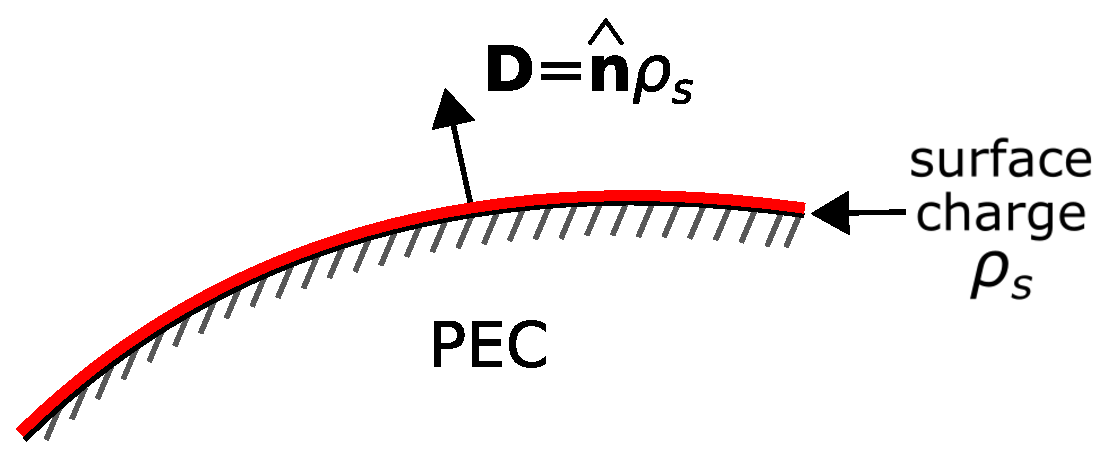
\includegraphics[width=2.5in]{modules/m0021_fPEC.eps}
% https://commons.wikimedia.org/wiki/File:M0021_fPEC.svg
}}{An arbitrary curved surface, labeled PEC. The outside of the surface is colored red, with lines extending at an angle inside the curve of the surface. It is labeled "surface charge rho sub s". An arrow points out of the surface at a perpendicular angle and is labeled bold D = n-hat * rho sub s. }
\end{center} 
\centerline{\scriptsize 
\copyright~\hyperref[m0021_fPEC_Credit]{K.\ Kikkeri} 
\href{https://creativecommons.org/licenses/by-sa/4.0/}{CC BY~SA 4.0} 
} 
\caption{
\label{m0021_fPEC}
The component of ${\bf D}$ that is perpendicular to a perfectly-conducting surface is equal to the charge density on the surface.
}
\end{figure}
%
In Section~\ref{m0020_Boundary_Conditions_on_E}, we established that the tangential component of the electric field must be zero, and therefore, the electric field is directed entirely in the direction perpendicular to the surface.
We further know that the electric field within the conductor is identically zero.
Therefore, ${\bf D}$ at any point on $\mathcal{S}$ is entirely in the direction perpendicular to the surface and pointing into the non-conducting medium.
However, it is also possible to determine the magnitude of ${\bf D}$.
We shall demonstrate in this section that  
%
%ORB HIGHLIGHT
\begin{mdframed}[backgroundcolor=yellow!20,nobreak=true] 
At the surface of a perfect conductor, the magnitude of {\bf D} is equal to the surface charge density $\rho_s$ (units of C/m$^2$) at that point.
\end{mdframed}
%
The following equation expresses precisely the same idea, but includes the calculation of the perpendicular component as part of the statement:
%
\begin{equation}
{\bf D} \cdot \hat{\bf n} = \rho_s~~\mbox{(on PEC surface)}
\label{m0021_eEPECBC}
\end{equation} 
%
where $\hat{\bf n}$ is the normal to ${\mathcal S}$ pointing into the non-conducting region.
(Note that the orientation of $\hat{\bf n}$ is now important;  we have assumed $\hat{\bf n}$ points into region~1, and we must now stick with this choice.)
Before proceeding with the derivation, it may be useful to note that this result is not surprising.  The very definition of electric flux (Section~\ref{m0011_Electric_Flux_Density}) indicates that ${\bf D}$ should correspond in the same way to a surface charge density.  
However, we can show this rigorously, and in the process we can generalize this result to the more-general case in which neither of the two materials are PEC.

The desired more-general boundary condition may be obtained from the integral form of Gauss' Law (Section~\ref{m0014_Gauss_Law_Integral_Form}), as illustrated in Figure~\ref{m0021_fGL}.
%
\begin{figure}
\begin{center}
\pdftooltip{{  % note double braces
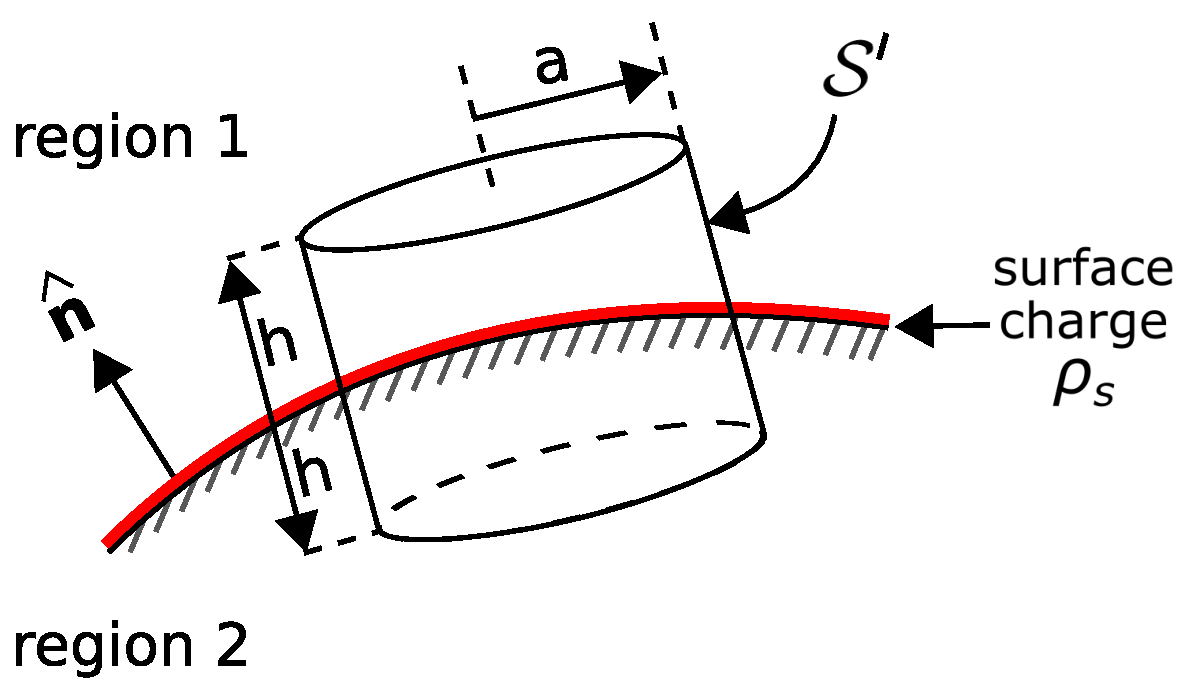
\includegraphics[width=2.5in]{modules/m0021_fGL.eps}
% https://commons.wikimedia.org/wiki/File:M0021_fGL.svg
}}{An arbitrary surface with a surface charge rho sub s. A cylinder drawn with it's midpoint intersecting at a perpendicular angle with the surface. Further details in text.}
\end{center} 
\centerline{\scriptsize 
\copyright~\hyperref[m0021_fGL_Credit]{K.\ Kikkeri} 
\href{https://creativecommons.org/licenses/by-sa/4.0/}{CC BY~SA 4.0} 
} 
\caption{
\label{m0021_fGL}
Use of Gauss' Law to determine the boundary condition on ${\bf D}$.
}
\end{figure}
%
Let the surface of integration $\mathcal{S}'$ take the form of closed cylinder centered at a point on the interface and for which the flat ends are parallel to the surface and perpendicular to $\hat{\bf n}$.  Let the radius of this cylinder be $a$, and let the length of the cylinder be $2h$.  From Gauss' Law we have
%
\begin{align}
\oint_{{\mathcal S}'}{ {\bf D} \cdot d{\bf s} } &= \int_{top} { {\bf D} \cdot d{\bf s} } &            \nonumber \\
                                                 &+ \int_{side} { {\bf D} \cdot d{\bf s} } &            \nonumber \\
                                                 &+ \int_{bottom} { {\bf D} \cdot d{\bf s} } &= Q_{encl} 
\end{align}
%
where 
the ``top'' and ``bottom'' are in Regions~1 and 2, respectively, and
$Q_{encl}$ is the charge enclosed by ${\mathcal S}'$.
Now let us reduce $h$ and $a$ together while (1) maintaining a constant ratio $h/a\ll 1$ and (2) keeping $\mathcal{S}'$ centered on $\mathcal{S}$.
Because $h\ll a$, the area of the side can be made negligible relative to the area of the top and bottom.
Then as $h\to 0$ we are left with  
%
\begin{equation}
\int_{top} { {\bf D} \cdot d{\bf s} } + \int_{bottom} { {\bf D} \cdot d{\bf s} }  \to Q_{encl} 
\end{equation}
%
As the area of the top and bottom sides become infinitesimal, the variation in ${\bf D}$ over these areas becomes negligible.  Now we have simply: 
%
\begin{equation}
{\bf D}_1 \cdot \hat{\bf n}\Delta A + {\bf D}_2 \cdot \left( -\hat{\bf n} \right) \Delta A \to Q_{encl} 
\end{equation}
%
where ${\bf D}_1$ and ${\bf D}_2$ are the electric flux density vectors in medium~1 and medium~2, respectively,
and $\Delta A$ is the area of the top and bottom sides.  
The above expression can be rewritten
%
\begin{equation}
\hat{\bf n} \cdot \left( {\bf D}_1 - {\bf D}_2 \right) \to
\frac{ Q_{encl} }{\Delta A}   
\end{equation}
%
Note that the left side of the equation must represent a actual, physical surface charge; this is apparent from dimensional analysis and the fact that $h$ is now infinitesimally small.  Therefore:
%
\begin{equation}
\boxed{
\hat{\bf n} \cdot \left( {\bf D}_1 - {\bf D}_2 \right) = \rho_s
}
\label{m0021_eBCD}
\end{equation}       
%
where, as noted above, $\hat{\bf n}$ points into region~1.
Summarizing:
%
%ORB HIGHLIGHT
\begin{mdframed}[backgroundcolor=yellow!20,nobreak=true] 
Any discontinuity in the normal component of the electric flux density across the boundary between two material regions is equal to the surface charge.
\end{mdframed}

Now let us verify that this is consistent with our preliminary finding, in which Region~2 was a PEC.
In that case ${\bf D}_2=0$, so we see that Equation~\ref{m0021_eEPECBC} is satisfied, as expected.
If neither Region~1 nor Region~2 is PEC \emph{and} there is no surface charge on the interface, then we find 
$\hat{\bf n} \cdot \left( {\bf D}_1 - {\bf D}_2 \right)=0$; i.e.,
%
%ORB HIGHLIGHT
\begin{mdframed}[backgroundcolor=yellow!20,nobreak=true] 
In the absence of surface charge, the normal component of the electric flux density must be continuous across the boundary.
\end{mdframed}

Finally, we note that since ${\bf D}=\epsilon{\bf E}$, Equation~\ref{m0021_eBCD} implies the following boundary condition on ${\bf E}$:
%
\begin{equation}
\hat{\bf n} \cdot \left( \epsilon_1{\bf E}_1 - \epsilon_2{\bf E}_2 \right) = \rho_s
\label{m0021_eBCE}
\end{equation} 
%
where $\epsilon_1$ and $\epsilon_2$ are the permittivities in Regions~1 and 2, respectively.
The above equation illustrates one reason why we sometimes prefer the ``flux'' interpretation of the electric field to the ``field intensity'' interpretation of the electric field.




